\documentclass{ctexart}
\usepackage{xcolor}
\usepackage{setspace}
\usepackage{tikz}
\usepackage{ctex}
\usepackage{geometry}
\usepackage{amsmath}
\usepackage{graphicx} 
\usepackage{subfigure}
\usepackage{float}
\usepackage{algorithm}  
\usepackage{algorithmicx}  
\usepackage{algpseudocode} 
\usepackage{url}
\usepackage{amsthm, amssymb, appendix, bm, graphicx, hyperref, mathrsfs}
\usepackage{tabularx}
\usepackage{booktabs} %需要加载宏包{booktabs}
\usepackage{multirow}
\usepackage{diagbox} % 加载宏包
\usepackage{pifont}

\usepackage{siunitx}
\usepackage{listings}
\usepackage{float}
\pagestyle{plain}

\usetikzlibrary{datavisualization}
\usetikzlibrary{arrows,shapes,chains}
\usepackage{listings}
\lstset{language=C++}
\lstset{breaklines}
\lstset{extendedchars=false}
\lstset{numbers=left}
\geometry{a4paper,left=2.5cm,right=2.5cm,top=2.5cm,bottom=2.5cm}
\CTEXsetup[format={\Large\bfseries\centering}]{section}
\tikzstyle{startstop} = [rectangle,rounded corners, minimum width=3cm,minimum height=1cm,text centered, text width=6cm,draw=black]
\tikzstyle{io} = [trapezium, trapezium left angle = 70,trapezium right angle=110,minimum width=5cm,minimum height=1cm,text centered,draw=black,fill=white]
\tikzstyle{process} = [rectangle,minimum width=3cm,minimum height=1cm,text centered,text width =3cm,text width=6cm,draw=black]
\tikzstyle{decision} = [diamond,minimum width=3cm,minimum height=1cm,text centered,text width=6cm,aspect=2,draw=black,thin]
\tikzstyle{arrow} = [thick,->,>=stealth]
\renewcommand{\algorithmicrequire}{\textbf{Input:}}  % Use Input in the format of Algorithm  
\renewcommand{\algorithmicensure}{\textbf{Output:}} % Use Output in the format of Algorithm  
\newcommand{\subsubsubsection}[1]{\paragraph{#1}\mbox{}\\}
\setcounter{secnumdepth}{4} % how many sectioning levels to assign numbers to
\setcounter{tocdepth}{4} % how many sectioning levels to show in ToC
\begin{document}

\section{模型假设}
1. \quad 基于自身感知的高度信息,本文默认无人机均保持在同一个高度上飞行,即所有无人机在同一个平面上。

2. \quad 假设第一问中的所有小问9架无人机理论上都应均匀分布在半径为100m的圆周上。

3. \quad 假设无人机接收到的方向信息不存在误差。


\subsection{问题一模型的建立与求解}


  \subsubsection{二分移动路径法}

  首先我们需要确定圆周上的每架无人机到原点的连线和x轴的夹角大小,现在以编号为$FY02$的无人机为例说明如何确定该夹角大小。

  设$FY1,FY2$分别为$FY01$和$FY02$的理想位置,$FY1^{'},FY2^{'}$分别为$FY01$和$FY02$的真实位置,坐标原点为$O$,则$\alpha$为$OFY1^{'}$和$OFY2^{'}$两边的初始夹角。设$FY2^{''}$是$FY02$调整后的位置,则$\alpha^{'}$为$OFY1^{'}$和$OFY2^{''}$的夹角。
  若有$\alpha = \alpha^{'}$,说明$FY2^{''}$在$OFY2^{'}$的延长线上。令$FY2^{''}$在以$FY2^{'}$为圆心,常数$r$(具体实现时设置为$1m$)为半径的圆上调整。尽管我们初始时无法知道$FY2^{'}$的精确位置,但通过$r$和$\theta$容易计算$FY2^{'}$到$FY2^{‘'}$的变化量,故可以使用形式为$(\Delta x,\Delta y)$的调整指令使无人机在圆周上调整。
  
  设$FY2^{''}FY2^{'}$与x轴的夹角为$\theta$,则$\theta$和$\alpha^{'}$之间存在一个函数映射关系$\alpha^{'}=f(\theta)$,那么$FY2^{'}$的方向确定问题就转化为了$\alpha=f(\theta)$的方程求解问题。根据$FY02$的理想位置划定$\theta$的大致区间$[40^{\circ}-20^{\circ},40^{\circ}+20^{\circ}]$后,不难发现在此范围内$f(\theta)$是单调的,那么我们就可以使用二分法求解$\alpha=f(\theta)$。

  \begin{figure}[H]
    \centering
    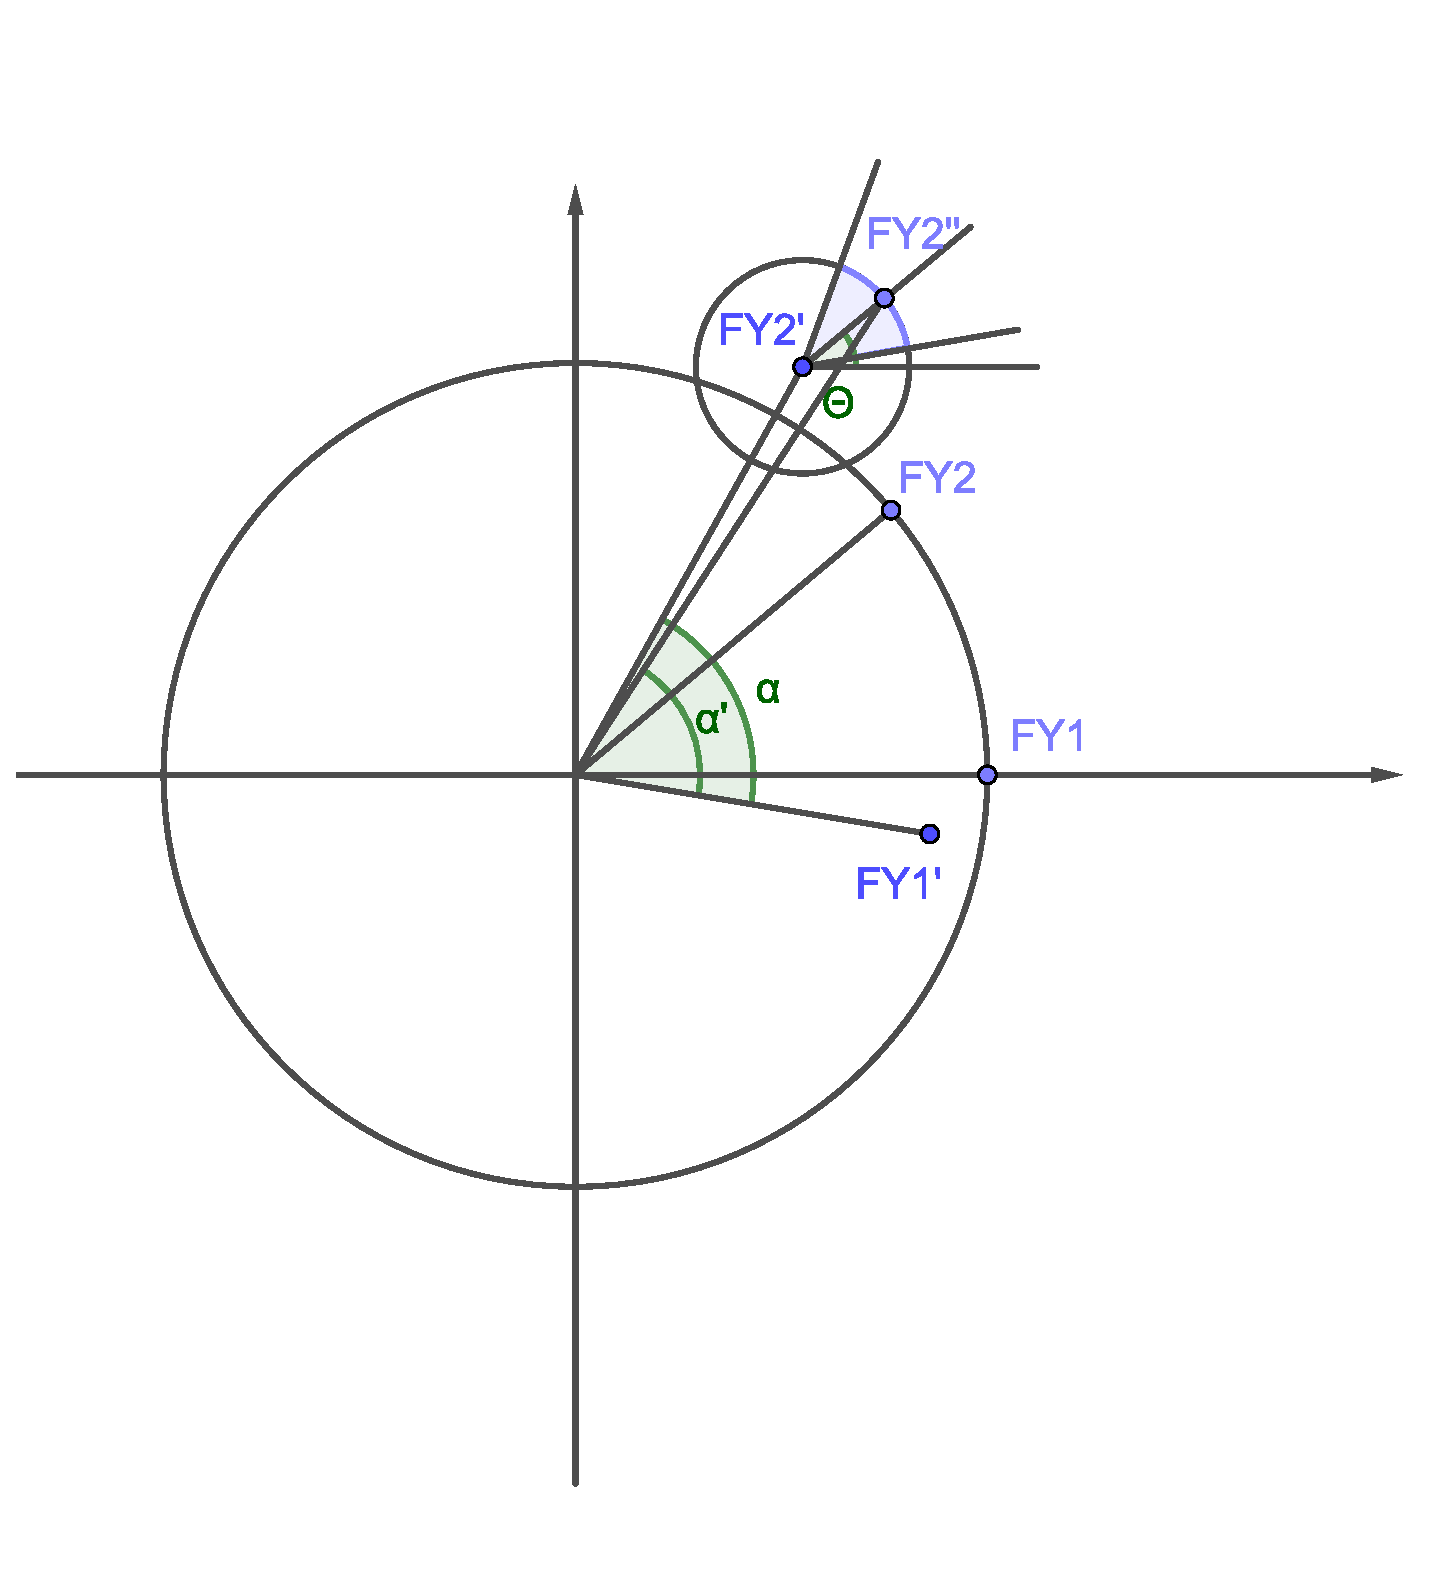
\includegraphics[width=0.45\linewidth]{pic/bisection.eps}
    \caption{二分移动路径法示意图}
    \label{二分移动路径法示意图}
    \end{figure}


    我们可以对其他编号的无人机根据其理想位置确定不同的$\theta$范围,在各自的范围内分别二分移动路径,最终确定各自位置到原点的连线和x轴的夹角大小。

  \subsubsection{二分移动路径法}
    在锥形编队队形下,我们可以通过控制其他无人机到$FY01$的连线与$FY01-FY05$连线的夹角大小,二分确定其他无人机的方向,具体二分方法和问题一的第3小问的方法类似,但由于$FY01$可以作为接收点,我们可以直接得到夹角的角度信息,而不是通过三角形内其他两个角的角度,间接计算夹角。
  \subsubsection{结论说明}
    当需要定位的无人机偏差过大时,如$FY08$偏差到了$FY01-FY05$连线下方,则会使其丧失可二分性,可能导致求解失败。当偏差较小时,则可以在共$20$轮询问和调整后,将每个无人机的角度偏差降低到$10^{-5}$以内。

\section{模型的评价与推广}
\subsection{模型的优点}
    \begin{itemize}
      \item 定位精度高,问题一(1)的定位误差可基本控制在$10^{-8}m$内,问题一(2)(3)的定位误差和累积误差可基本控制在$10^{-4}m$内。
      \item 使用无人机接收到的角度信息验证定位准确性,可以在实际应用时进行检验,不需要得知真实坐标,适用性强,且在计算机模拟时检验结果和用真实坐标的检验结果相同,正确性高。
      \item 投票机制让定位错误率大大下降,同时尽量使用了少的发射无人机进行定位,且投票机制衍生出的二轮投票机制可以进一步延伸,得到使用三架甚至更多未知编号的发射无人机进行定位的多轮投票模型,进一步提高定位精度和正确率。
    \end{itemize}
\subsection{模型的缺点}
    \begin{itemize}
      \item 当需要定位的无人机距离其理想位置偏差较大时,模型可能出现定位错误的情况。
      \item 基准无人机需要处理的角度信息远多于其他无人机,对其计算性能和精度要求较高。
      \item 在投票模型中计算误差圆对应的角度范围时使用了较为方便实现的蒙特卡洛方法,精度较低且复杂度较高,可以考虑改用论文提到的计算几何相关的计算方法。
      \item 在最后一次调整到接近理想位置之前,在前期二分调整时,各无人机可能会先远离理想位置。
    \end{itemize}
\subsection{模型的推广}
    问题一(1)中的定位模型可以推广到用平面上任意3个已知位置的发射源及接收点得到的角度信息来定位一个已知大致位置的接收点,不必局限在圆周附近进行定位。

    问题一(3)和问题二中先二分确定角度,再解三角形确定距离以定位每个无人机和基准无人机的相对位置的思路也可以拓展到其他编队队形的调整上。

    



\end{document}